% 1. Pass options BEFORE documentclass to prevent clashes
\PassOptionsToPackage{numbers, compress}{natbib}
\PassOptionsToPackage{table}{xcolor} % Handles the [table] option for xcolor early

\documentclass{article}

% 2. NeurIPS Style (ensure the .sty file is named exactly this in your folder)
\usepackage[final]{neurips_2026}

% 3. Graphics and Visualization
\usepackage{graphicx}
\usepackage{tikz}
\usetikzlibrary{positioning, arrows.meta, shapes.geometric}
\usepackage{adjustbox}
\usepackage{rotating}

% 4. Math and Symbols
\usepackage{amsmath, amssymb, amsfonts}
\usepackage{nicefrac}
\usepackage{microtype}
\usepackage{siunitx}

% 5. Tables and Layout
\usepackage{multirow}
\usepackage{listings}
\lstset{
    basicstyle=\ttfamily\small,
    breaklines=true,
    frame=single,
    columns=fullflexible
}
\usepackage{booktabs}   % Only load once
\usepackage{tabularx}
\usepackage{array}
\usepackage{float}
\usepackage{placeins}
\usepackage{caption}

% 6. Algorithms
\usepackage{algorithm}
\usepackage{algpseudocode}

% 7. Miscellaneous
\usepackage[utf8]{inputenc}
\usepackage[T1]{fontenc}
\usepackage{url}

% 8. Hyperref (Usually load this LAST to avoid link errors)
\usepackage{hyperref}

% --- REMOVED: \usepackage[numbers]{natbib} (Redundant/Causes Error) ---

\title{Do earnings call transcripts predict post-announcement returns?\\
 \vspace{0.2cm} \textnormal{\large An NLP-based approach on Russell 1000 equities}}

% Note: NeurIPS 'final' mode usually hides the date, but it's fine for an ENSAE project.
% NeurIPS style author block
\author{%
  Matéo Molinaro \\
  ENSAE Paris \\
  \texttt{mateo.molinaro@ensae.fr} \\
  \And
  Pierre Chuzeville \\
  ENSAE Paris \\
  \texttt{pierre.chuzeville@ensae.fr} \\
}

\begin{document}
\maketitle

\begin{abstract}
This paper investigates whether earnings call transcripts contain information that is predictive of post-announcement idiosyncratic stock returns. We construct a systematic machine learning pipeline that transforms raw transcript text into quantitative signals and evaluates their out-of-sample forecasting performance on the Russell~1000 universe. We extract two families of text representations, sparse TF-IDF bag-of-words features on preprocessed transcripts, and dense semantic embeddings from the pre-trained sentence transformer \textit{all-MiniLM-L6-v2}, and combine them with traditional finance-specific sentiment scores derived from the Loughran--McDonald dictionary. For each earnings event, targets are defined as multi-horizon cumulative idiosyncratic returns (residuals from a rolling CAPM estimated exclusively on pre-filing data) at horizons of 1, 3, 5 and 21 trading days. Model training and evaluation follow a strict quarterly walk-forward cross-validation scheme that eliminates forward-looking bias by design. We compare three feature compositions across four regression models (Ridge, Lasso, Random Forest, Gradient Boosting) and evaluate performance using directional accuracy, long--short spread, and an interpretable excess-RMSE relative to the CAPM null model. This framework allows us to systematically identify which combination of text representation, prediction horizon, and model architecture extracts the most economically meaningful signals from earnings calls.
\end{abstract}

\tableofcontents
\newpage

% ============================================================
\section{Introduction (Matéo)}
% ============================================================

Earnings call transcripts are among the richest sources of forward-looking corporate information available to investors. Each quarter, executives discuss financial performance, strategic priorities, and the business outlook in a format that is simultaneously structured enough for systematic analysis and nuanced enough to contain signals unlikely to be fully impounded in price the moment the call concludes. The post-earnings-announcement drift (PEAD) literature has documented that markets take time to incorporate even the quantitative earnings surprise into prices; the question of whether the \textit{qualitative} content of the call carries additional predictive power remains an active area of research.\\

This project contributes to this literature by constructing a complete, end-to-end pipeline that transforms raw transcript text into out-of-sample idiosyncratic stock return forecasts for the Russell~1000 universe. Three main questions structure the analysis. First, do different ways of representing transcript text---from classical bag-of-words to modern neural sentence embeddings---differ in their ability to predict post-announcement returns? Second, which prediction horizon (the immediate price reaction, the weekly or monthly drift) is most amenable to text-based forecasting? Third, do NLP features add incremental value on top of the classical finance-specific sentiment indicators derived from the Loughran--McDonald word list?\\

The pipeline proceeds in four steps. First, we construct the prediction target: for each earnings event, the cumulative idiosyncratic return at multiple forward horizons is computed from a rolling CAPM estimated strictly on data available before the filing date, ensuring no forward-looking bias. Second, each transcript is encoded into three families of features---TF-IDF sparse vectors, dense sentence-transformer embeddings, and traditional dictionary-based sentiment scores---assembled into three feature compositions spanning the trade-off between interpretability and expressive power. Third, a quarterly walk-forward cross-validation scheme selects hyperparameters and retrains models at each rebalancing date. Fourth, out-of-sample predictions are evaluated against metrics that capture directional accuracy, long--short economic profitability, and excess predictive power relative to the CAPM null model.\\

The project is implemented in Python and the full source code is available on GitHub.\footnote{\url{https://github.com/mateomolinaro1/NLPQuantStrat}} Data are loaded from Amazon S3 via a bespoke data management layer that handles return alignment, NaN policies, and transcript preprocessing.


% ============================================================
\section{Related Work (Pierre)}
% ============================================================

\paragraph{Post-earnings-announcement drift.}
The existence of predictable return patterns following earnings announcements, commonly called PEAD, is one of the anomalies in the asset pricing literature \cite{ball1968}. Prices fail to adjust immediately to the information conveyed by the earnings surprise, giving rise to a drift that can persist for months. The magnitude and persistence of PEAD motivate the use of earnings-period information, including the textual content of the accompanying call, as a basis for systematic return prediction.

\paragraph{Textual analysis in finance.}
Tetlock~\cite{tetlock2007} showed that the fraction of negative words in Wall Street Journal columns predicts near-term market-level returns, establishing that linguistic sentiment carries price-relevant information. Loughran and McDonald~\cite{lm2011} challenged the application of generic sentiment dictionaries to financial texts, demonstrating that domain-specific word lists perform substantially better in financial documents. Their dictionary, tuned to the particular language of corporate filings and calls, has since become the standard reference for dictionary-based financial sentiment analysis.

\paragraph{NLP applied to earnings calls.}
Earnings call transcripts have been used to predict both short-run returns and longer-term accounting outcomes. Early work focused on tone, the ratio of positive to negative words, and showed that a more positive tone in the prepared remarks is associated with better subsequent stock performance, while uncertainty in the Q\&A section is associated with adverse outcomes \cite{kearney2014}. More recent approaches apply neural text representations to capture meaning beyond simple word counting: bidirectional transformers, in particular, have been applied to 8-K filings and earnings call transcripts to predict stock returns at various horizons, with mixed but generally positive results \cite{yang2020finbert}.

\paragraph{Walk-forward validation in ML finance.}
A key methodological concern in applying machine learning to financial data is the avoidance of look-ahead bias. The standard i.i.d.\ cross-validation framework is inappropriate because financial observations are serially correlated and future data leaks into the training set when folds are assigned randomly. Walk-forward (or expanding-window) validation, in which the model is always trained on data up to a given date and evaluated on the subsequent period, is the standard remedy \cite{lopez2018}. Our framework follows this convention and additionally introduces a buffer between the validation and test windows to prevent the long-horizon targets of validation events from overlapping with the test period.


% ============================================================
\section{Data (Pierre)}
% ============================================================

\subsection{Asset universe and market data}

The equity universe consists of Russell~1000 index constituents, providing a large-cap and mid-cap U.S. equity panel with good liquidity and broad sector coverage. Daily total returns for index constituents are sourced from a CRSP/WRDS. The benchmark return series is the Russell~1000 total return index sourced on BBG. The risk-free rate is the daily U.S. one-month Treasury bill rate retived from the FRED website. All three series are aligned to the daily dates of the assets' returns: the risk-free rate and benchmark are forward-filled by up to five calendar days to handle public holidays and minor reporting gaps; asset returns are kept without filling to avoid artificially reducing return volatility.

\subsection{Earnings call transcripts}

Earnings call transcripts (called from the Ninja API) are matched to their corresponding \textit{(filing date, asset)} pair through a mapping table that links each transcript to its asset identifier and the date on which the earnings call was held. Two versions of each transcript are available:
\begin{itemize}
  \item \texttt{transcript}: the full unprocessed text of the call, retaining punctuation, capitalization, and stop words. Used as input to the sentence-transformer encoder, which is designed to operate on natural language.
  \item \texttt{transcript\_cleaned}: a preprocessed version obtained by lowercasing, removing stop words, and applying Porter stemming. Used as input to TF-IDF to reduce vocabulary noise.
\end{itemize}
On average, most quarters from 2015 to 2025 contain between 800 and 1,000 transcripts, providing a robust statistical foundation, see Figure [\ref{fig:nber_transcripts}].

Each event is represented by exactly one (filing\_date, asset) pair. Duplicate entries (e.g., multiple recordings of the same call) are resolved by keeping the last available text.


\subsection{Loughran--McDonald sentiment dictionary}

Traditional sentiment features are computed using the Loughran--McDonald financial sentiment dictionary \cite{lm2011}, which provides time-stamped positive, negative, and uncertainty word lists designed specifically for corporate financial language. To avoid look-ahead bias in the dictionary itself, a yearly version is constructed: for any transcript filed in year~$t$, only words that had been added to the dictionary on or before year~$t$ are counted. This ensures that the sentiment scores are fully point-in-time.


% ============================================================
\section{Methodology}
% ============================================================

\subsection{Target construction: idiosyncratic returns (Matéo)}

\subsubsection{Motivation}

Raw stock returns conflate firm-specific information with market-wide and sector-wide movements. A transcript-based signal is inherently a firm-level signal and should therefore be evaluated against a firm-level return. We use CAPM idiosyncratic returns---residuals with respect to the market factor---as the prediction target, which has two practical advantages. First, idiosyncratic returns are \textbf{approximately} zero-mean by construction (since $\mathbb{E}[\alpha_i] \approx 0$ in an \textbf{efficient} market at the cross-sectional level), which makes the null-model baseline mathematically clean (see Section~\ref{sec:metrics}). Second, purging the common market component reduces noise that is uninformative for a firm-level text signal and improves the signal-to-noise ratio of the prediction task.

\subsubsection{Rolling CAPM betas}

For each asset $i$ and each calendar date $t$, we estimate a rolling ordinary least squares beta using a window of $W = 252$ trading days (approximately one year):

\begin{equation}
\hat{\beta}_i(t)
= \frac{\widehat{\mathrm{Cov}}\!\left[r_i(s) - r_f(s),\; r_m(s) - r_f(s)\right]_{s \in [t-W+1,\,t]}}
       {\widehat{\mathrm{Var}}\!\left[r_m(s) - r_f(s)\right]_{s \in [t-W+1,\,t]}},
\end{equation}

where $r_i(t)$ is the daily total return of asset $i$, $r_f(t)$ is the risk-free rate, and $r_m(t)$ is the benchmark (Russell~1000 CW) return. The beta is computed using data up to and including date~$t$, so it is available to an investor at date~$t+1$ without any forward-looking bias.

\subsubsection{Daily idiosyncratic returns}

The daily idiosyncratic return residual is:

\begin{equation}
\mathrm{idio}_i(t)
= \bigl(r_i(t) - r_f(t)\bigr)
  - \hat{\beta}_i(t-1)\,\bigl(r_m(t) - r_f(t)\bigr),
\end{equation}

where $\hat{\beta}_i(t-1)$ is the beta estimated through the previous trading day, so the return at date~$t$ is not used in its own beta computation.

\subsubsection{Multi-horizon cumulative targets}

For each earnings event filed at date~$t$ by company~$i$, the prediction target at horizon~$h$ is the cumulative idiosyncratic return over the $h$ trading days immediately following the filing date:

\begin{equation}
y^{(h)}_{i,t}
= \prod_{s=t+1}^{t+h} \bigl(1 + \mathrm{idio}_i(s)\bigr) - 1.
\end{equation}

The return window begins at $t+1$, the first post-call trading day, to avoid using intraday prices from the same day as the call (which would constitute look-ahead bias). We consider four horizons: $h \in \{1, 3, 5, 21\}$ trading days, corresponding approximately to one day, three days, one week and one month ahead. Events near the end of the return series will have \texttt{NaN} targets where insufficient forward data exist; these events are excluded from model training and evaluation but still receive predictions.

Table~\ref{tab:horizons} summarises the economic interpretation of each horizon.

\begin{table}[H]
\centering
\caption{Target horizons and their economic interpretation}
\label{tab:horizons}
\begin{tabular}{rll}
\toprule
\textbf{Horizon $h$} & \textbf{Calendar approx.} & \textbf{Economic story} \\
\midrule
1d  & 1 trading day  & Immediate market reaction to the call \\
3d & 3 days      & Mid week reaction \\
5d  & 1 week         & Short-run information absorption / momentum \\
21d & 1 month        & Medium-run drift (PEAD regime) \\
\bottomrule
\end{tabular}
\end{table}

\subsection{Text representations (Pierre)}

\subsubsection{TF-IDF bag-of-words features}

The Term Frequency--Inverse Document Frequency (TF-IDF) representation transforms each transcript into a weighted vector of token importance scores. A single \texttt{TfidfVectorizer} is fitted on the full corpus of preprocessed transcripts (\texttt{transcript\_cleaned}) and retains the top 200 tokens by corpus-level TF-IDF weight, using unigrams and bigrams ($n$-gram range $[1, 2]$). The resulting feature matrix has dimension 200, with columns labeled $\mathtt{tfidf\_0}$ through $\mathtt{tfidf\_199}$.

TF-IDF is computationally cheap, fully interpretable (each dimension corresponds to a specific token or bigram), and captures the relative importance of domain-specific vocabulary across the corpus. Its primary limitation is insensitivity to word order and inability to capture semantic similarity between synonymous expressions, a limitation addressed by the sentence-transformer approach below.

\subsubsection{Sentence-transformer dense embeddings}

Dense semantic embeddings are produced using the pre-trained sentence-transformer \textit{all-MiniLM-L6-v2}~\cite{reimers2019}, a compact 6-layer transformer fine-tuned on over one billion sentence pairs to produce semantically meaningful 384-dimensional embeddings. Earnings call transcripts far exceed the model's 512-subword-token context limit. We address this with a \textit{chunk-and-mean-pool} strategy: each transcript is split into non-overlapping word-level chunks of 256 words (approximately 300--500 subword tokens), each chunk is encoded independently, and the chunk embeddings are averaged into a single document vector:

\begin{equation}
\mathbf{e}_{\mathrm{doc}}
= \frac{1}{K}\sum_{k=1}^{K} f_\theta(\text{chunk}_k),
\end{equation}

where $K$ is the number of chunks and $f_\theta$ denotes the transformer encoder. Mean pooling treats all sections of the transcript as equally informative, which is a simplification but avoids the truncation artifacts of simply using the first 512 tokens. The resulting features are 384-dimensional vectors labeled $\mathtt{emb\_0}$ through $\mathtt{emb\_383}$, and are cached to S3 after computation so that the expensive inference step does not need to be repeated.

\subsubsection{Dictionary-based sentiment features}

Seventeen sentiment features are derived from applying the Loughran--McDonald dictionary to each transcript, divided into seven \emph{legacy} features (counts, polarity, density, and momentum) and ten newly designed \emph{alpha} features (ratios, temporal surprises, sentence-level statistics, and an interaction term). All are computed in a wide panel format (dates $\times$ assets) and then looked up for each earnings event:

\begin{table}[H]
\centering
\caption{Dictionary-based sentiment features}
\label{tab:sentiment_features}
\begin{tabular}{lp{9cm}}
\toprule
\textbf{Feature} & \textbf{Definition} \\
\midrule
\texttt{positive\_count}        & Number of positive-sentiment words in the transcript. \\
\texttt{negative\_count}        & Number of negative-sentiment words in the transcript. \\
\texttt{word\_count}            & Total word count, serving as a proxy for transcript length. \\
\texttt{polarity}               & Standardized sentiment score calculated as $(\text{positive} - \text{negative}) / \text{word\_count}$. \\
\texttt{sentiment\_density}     & Proportion of emotive content calculated as $(\text{positive} + \text{negative}) / \text{word\_count}$. \\
\texttt{pos\_polarity\_count\_q} & Rolling $q$-quarter ($q=4$) moving average of transcript polarity. \\
\texttt{polarity\_delta}        & Quarter-over-quarter change in raw polarity scores. \\
\texttt{pos\_ratio}             & Proportion of positive words relative to the total word count. \\
\texttt{neg\_ratio}             & Proportion of negative words relative to the total word count. \\
\texttt{unc\_ratio}             & Proportion of uncertainty-related words within the transcript. \\
\texttt{net\_sentiment}         & Normalized sentiment score, identified as a primary predictor of asset outperformance. \\
\texttt{sentiment\_surprise}    & Measure of unexpected sentiment relative to market or historical expectations. \\
\texttt{sentiment\_zscore}      & Sentiment surprise measured against the company's specific historical baseline. \\
\texttt{sentiment\_delta}       & Period-over-period change in sentiment, most potent immediately following transcript release. \\
\texttt{sent\_var}              & Statistical variability or complexity of the discourse throughout the transcript. \\
\texttt{toxic\_density}         & Concentration of highly negative language, showing a negative correlation with forward returns. \\
\texttt{sent\_vol\_interaction} & Interaction term between sentiment and market volume, representing a "conviction" signal boost. \\
\bottomrule
\end{tabular}
\end{table}

These features are interpretable and require no neural network inference, making them fast to compute. The momentum feature (\texttt{pos\_polarity\_count\_q}) captures whether the tone has been improving or deteriorating over the past year, while \texttt{polarity\_delta} captures sentiment surprises relative to the most recent quarter. Their joint limitation is insensitivity to context: they cannot distinguish negation, irony, or subtle forward-looking language.

\subsection{Feature composition modes (Pierre)}

Six feature compositions are defined (but only three will be studied due to computational reasons) to isolate the contribution of each representation family and study their interactions:

\begin{table}[H]
\centering
\caption{Feature composition modes}
\label{tab:modes}
\begin{tabular}{lcccc}
\toprule
\textbf{Mode} & \textbf{TF-IDF} & \textbf{Sent.-Transformer} & \textbf{Sentiment dict.} & \textbf{Dim.} \\
\midrule
\texttt{sentiment}           &            &            & \checkmark & 7   \\
\texttt{tfidf}               & \checkmark &            &            & 200 \\
\texttt{st}                  &            & \checkmark &            & 384 \\
\texttt{tfidf\_sentiment}    & \checkmark &            & \checkmark & 207 \\
\texttt{st\_sentiment}       &            & \checkmark & \checkmark & 391 \\
\texttt{all}                 & \checkmark & \checkmark & \checkmark & 591 \\
\bottomrule
\end{tabular}
\end{table}

Each mode defines a self-contained experiment: the feature matrix $X$ is assembled independently, NaN rows are dropped, and the walk-forward CV runs from scratch. Comparing \texttt{tfidf} vs.\ \texttt{tfidf\_sentiment} isolates the marginal value of dictionary features given TF-IDF; comparing \texttt{st} vs.\ \texttt{tfidf} isolates the value of semantic embeddings over bag-of-words; comparing \texttt{st\_sentiment} vs.\ \texttt{all} reveals whether TF-IDF adds anything once the transformer already captures the document semantics.

\subsection{Walk-forward cross-validation framework (Matéo)}
\label{sec:wfcv}

\subsubsection{Motivation}

Financial observations are serially dependent and their joint distribution is non-stationary. Standard i.i.d.\ cross-validation would severely overestimate out-of-sample performance by randomly assigning observations across folds and thereby leaking future return realizations into training data. We use a quarterly walk-forward scheme that is strictly out-of-sample by construction: at each rebalancing date, the model is trained exclusively on events that occurred before that date.

\subsubsection{Period layout}

The event panel is organized into calendar quarters. For each test quarter~$P$, the data are partitioned as follows:

\begin{equation}
\underbrace{[\;\text{train}\;]}_{\text{all past quarters}} \;\;
\underbrace{[\;\text{val}\;]}_{V \text{ quarters}} \;\;
\underbrace{[\;\text{buffer}\;]}_{B \text{ quarters}} \;\;
\underbrace{[\;P\;]}_{\text{test}}
\end{equation}

\begin{itemize}
  \item \textbf{Train}: all quarters preceding the validation window. An expanding window (default) uses all available history; a rolling window retains only the most recent $T$ quarters.
  \item \textbf{Validation} ($V = 1$ quarter): used exclusively for hyperparameter grid search. The scaler is fitted on train only and applied to validation, preventing distribution leakage.
  \item \textbf{Buffer} ($B = \lceil \max(h) / 63 \rceil$ quarters, automatically computed from the horizon set): a mandatory gap that prevents the forward-return window of the last validation event from extending into the test quarter. At $\max(h) = 63$ trading days, $B = 1$ quarter suffices.
  \item \textbf{Test} ($P$): events in the current quarter receive out-of-sample predictions from the model refitted on train $\cup$ val.
\end{itemize}

Figure~\ref{fig:wkfwd_schema} illustrates three successive test quarters, showing how the train window expands while val and buffer shift forward by one quarter each time.

\begin{figure}[H]
\centering
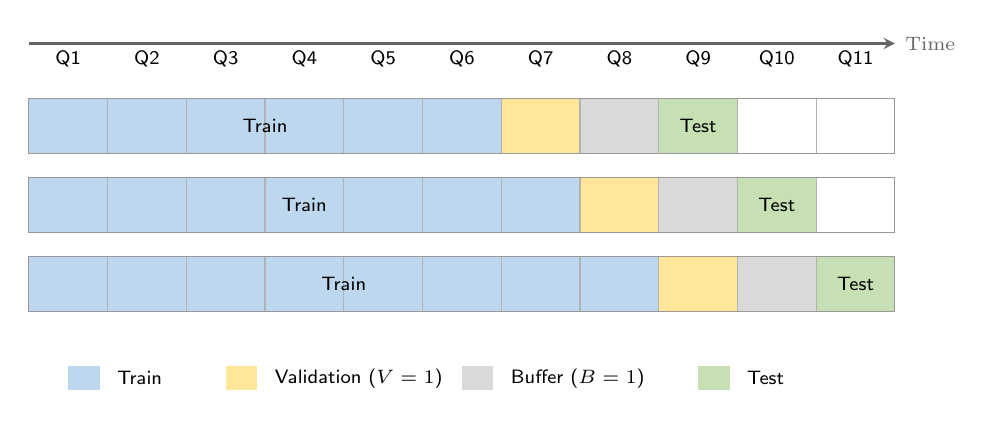
\begin{tikzpicture}[
    box/.style={rectangle, draw=black!50, minimum height=0.6cm, lw=0.4pt},
    label_node/.style={font=\scriptsize\sffamily},
    legend_node/.style={font=\scriptsize\sffamily, anchor=west}
]

  % --- Color Definitions ---
  \definecolor{ctrain}{RGB}{189, 215, 238} % Professional Blue
  \definecolor{cval}{RGB}{255, 230, 153}   % Professional Yellow
  \definecolor{cbuf}{RGB}{217, 217, 217}   % Soft Gray
  \definecolor{ctest}{RGB}{198, 224, 180}  % Professional Green

  % --- Time Axis (Q1 - Q11) ---
  \foreach \q in {1,...,11} {
    \node[label_node] at (\q-0.5, 3.2) {Q\q};
  }
  \draw[->, >=stealth, thick, black!60] (0, 3.4) -- (11, 3.4) node[right, font=\scriptsize] {Time};

  % --- Row 1: Test = Q9 ---
  \begin{scope}[shift={(0, 2)}]
    \fill[ctrain] (0,0) rectangle (6, 0.7);
    \fill[cval]   (6,0) rectangle (7, 0.7);
    \fill[cbuf]   (7,0) rectangle (8, 0.7);
    \fill[ctest]  (8,0) rectangle (9, 0.7);
    \foreach \x in {0,...,11} \draw[black!30] (\x, 0) -- (\x, 0.7);
    \draw[black!40] (0,0) rectangle (11, 0.7);
    \node[label_node] at (3, 0.35) {Train};
    \node[label_node] at (8.5, 0.35) {Test};
  \end{scope}

  % --- Row 2: Test = Q10 ---
  \begin{scope}[shift={(0, 1)}]
    \fill[ctrain] (0,0) rectangle (7, 0.7);
    \fill[cval]   (7,0) rectangle (8, 0.7);
    \fill[cbuf]   (8,0) rectangle (9, 0.7);
    \fill[ctest]  (9,0) rectangle (10, 0.7);
    \foreach \x in {0,...,11} \draw[black!30] (\x, 0) -- (\x, 0.7);
    \draw[black!40] (0,0) rectangle (11, 0.7);
    \node[label_node] at (3.5, 0.35) {Train};
    \node[label_node] at (9.5, 0.35) {Test};
  \end{scope}

  % --- Row 3: Test = Q11 ---
  \begin{scope}[shift={(0, 0)}]
    \fill[ctrain] (0,0) rectangle (8, 0.7);
    \fill[cval]   (8,0) rectangle (9, 0.7);
    \fill[cbuf]   (9,0) rectangle (10, 0.7);
    \fill[ctest]  (10,0) rectangle (11, 0.7);
    \foreach \x in {0,...,11} \draw[black!30] (\x, 0) -- (\x, 0.7);
    \draw[black!40] (0,0) rectangle (11, 0.7);
    \node[label_node] at (4, 0.35) {Train};
    \node[label_node] at (10.5, 0.35) {Test};
  \end{scope}

  % --- Legend ---
  \begin{scope}[shift={(0.5, -1)}]
    \fill[ctrain] (0,0) rectangle (0.4, 0.3); \node[legend_node] at (0.5, 0.15) {Train};
    \fill[cval]   (2,0) rectangle (2.4, 0.3); \node[legend_node] at (2.5, 0.15) {Validation ($V=1$)};
    \fill[cbuf]   (5,0) rectangle (5.4, 0.3); \node[legend_node] at (5.5, 0.15) {Buffer ($B=1$)};
    \fill[ctest]  (8,0) rectangle (8.4, 0.3); \node[legend_node] at (8.5, 0.15) {Test};
  \end{scope}

\end{tikzpicture}
\caption{Expanding walk-forward CV schema. The training window expands chronologically, followed by a validation set, a buffer period to prevent data leakage, and the out-of-sample test quarter.}
\label{fig:wkfwd_schema}
\end{figure}
\FloatBarrier

\subsubsection{Hyperparameter selection and scaling}

For each (test period, horizon, model) combination, hyperparameters are selected by grid search on the validation split. Feature scaling (StandardScaler) is fitted on the training events only and applied to validation events before scoring, so that the distribution of the validation split does not leak into the scaler fit. The validation scoring function is the \textit{long--short score}:

\begin{equation}
\mathrm{LS}\text{-}\mathrm{score}
= \frac{1}{n_{\mathrm{val}}} \sum_{j \in \mathrm{val}}
  \mathrm{sign}(\hat{y}_j)\, y_j,
\label{eq:ls_score}
\end{equation}

which directly estimates the expected P\&L per unit long/short bet and is more economically meaningful than RMSE for a trading objective. If fewer than 5 events are available in the validation window, the first grid point is used without scoring.

\subsubsection{Final fit and prediction}

Once best hyperparameters are identified, a final model is fitted on the combined train $\cup$ val sample using a fresh scaler refitted on that combined window. Predictions are then generated for all test-period events, including those with \texttt{NaN} targets (the model still produces a score, but the event is excluded from metric computation). This two-phase scaling (search scaler on train; final scaler on train $\cup$ val) maximises the data used for the final model while ensuring that neither phase involves information from the test period.

\subsubsection{Minimum data requirements}

A (period, horizon, model) combination is skipped if fewer than 50 non-NaN training events exist (\texttt{MIN\_TRAIN\_EVENTS}). The CV does not begin until at least 8 calendar quarters of history have accumulated (\texttt{MIN\_TRAIN\_PERIODS}), reflecting the 252-day rolling beta window: predictions from early periods would rely on unreliable betas and are excluded to avoid contaminating the evaluation.

\subsection{Forecasting models (Matéo)}
\label{sec:models}

Four regression models from scikit-learn are compared, spanning a range of complexity and inductive bias:

\begin{table}[H]
\centering
\caption{Forecasting models and hyperparameter grids}
\label{tab:models}
\begin{tabular}{llp{7.0cm}}
\toprule
\textbf{Model} & \textbf{Category} & \textbf{Hyperparameter grid} \\
\midrule
Ridge        & Regularized linear        & $\alpha \in \{0.01,\, 0.1,\, 1.0\}$ \\[0.3em]
Lasso        & Regularized linear (sparse) & $\alpha \in \{0.01,\, 0.1,\, 1.0\}$ \\[0.3em]
Random Forest    & Ensemble (bagging)    &
  $n\_\text{est.} \in \{100,\,200\}$;\;
  $\text{max\_depth} \in \{3,\,5\}$ \\[0.3em]
Gradient Boosting & Ensemble (boosting) &
  $n\_\text{est.} \in \{100,\,200\}$;\;
  $\text{max\_depth} \in \{3,\,5\}$;\;
  $\text{lr} \in \{0.05,\,0.1\}$ \\
\bottomrule
\end{tabular}
\end{table}

Ridge and Lasso serve as well-regularized linear baselines appropriate for high-dimensional feature spaces (TF-IDF, sentence-transformer). Lasso's $\ell_1$ penalty additionally performs implicit feature selection, which may be beneficial when few of the 200 or 384 dimensions carry genuine predictive signal. Random Forest and Gradient Boosting capture non-linear interactions at the cost of higher computational overhead; in high dimensions they are also more prone to overfitting, making the val-set grid search critical. All models are cloned at each fold using \texttt{sklearn.base.clone} to ensure complete independence between folds.

\subsection{Evaluation metrics (Matéo)}
\label{sec:metrics}

Out-of-sample performance is evaluated per (quarter, model, horizon) triplet using the following metrics, which together characterize both statistical and economic quality.

\subsubsection{Hit rate}

\begin{equation}
\mathrm{HitRate} = \frac{1}{n} \sum_{j=1}^{n} \mathbf{1}\!\left[\mathrm{sign}(\hat{y}_j) = \mathrm{sign}(y_j)\right].
\end{equation}

The natural baseline is 50\% (random directional guessing). Values above 50\% indicate consistent directional skill.

\subsubsection{Long--short spread}

We form a long leg (events with $\hat{y}_j > 0$) and a short leg ($\hat{y}_j < 0$) and compute:

\begin{equation}
\mathrm{Spread} = \bar{y}_{\mathrm{long}} - \bar{y}_{\mathrm{short}},
\end{equation}

where $\bar{y}$ denotes the mean realized idiosyncratic return of the respective leg. A positive spread indicates that the signal correctly ranks events by subsequent return. Statistical significance is assessed via the $t$-statistic:

\begin{equation}
t = \frac{\overline{\mathrm{MSR}}}{\widehat{\sigma}(\mathrm{MSR})/\sqrt{n}},
\end{equation}

where $\mathrm{MSR}_j = \mathrm{sign}(\hat{y}_j)\, y_j$ is the signed return per event, $\overline{\mathrm{MSR}}$ is its mean, and $\widehat{\sigma}$ its empirical standard deviation. This $t$-statistic is equivalent to a one-sample $t$-test of whether the mean signed return is zero.

\subsubsection{Mean signed return (long--short score)}

\begin{equation}
\mathrm{MSR} = \frac{1}{n}\sum_{j=1}^{n} \mathrm{sign}(\hat{y}_j)\,y_j,
\end{equation}

identical to the validation scorer (equation~\ref{eq:ls_score}). MSR can be interpreted as the expected return per unit of capital deployed in a long/short strategy that bets one unit on the predicted direction of each event. The baseline is 0 (no directional skill).

\subsubsection{Excess RMSE}

The standard RMSE is difficult to interpret in isolation because its absolute magnitude depends on the scale of idiosyncratic returns, which varies across assets and horizons. We define instead an \textit{excess RMSE}:

\begin{equation}
\mathrm{ExcessRMSE} = \mathrm{RMSE} - \sigma(y),
\end{equation}

where $\sigma(y) = \sqrt{\frac{1}{n}\sum_{j=1}^{n} y_j^2}$ is computed with $\mathrm{ddof}=0$.

The key property is that the null model---always predicting zero---achieves $\mathrm{ExcessRMSE} = 0$ exactly. Because idiosyncratic returns are approximately zero-mean by the CAPM construction ($\bar{y} \approx 0$):

\begin{equation}
\mathrm{RMSE}_{\hat{y}=0}
= \sqrt{\frac{1}{n}\sum_{j} (y_j - 0)^2}
= \sqrt{\frac{1}{n}\sum_{j} y_j^2}
= \sigma(y),
\end{equation}

so $\mathrm{ExcessRMSE}_{\hat{y}=0} = \sigma(y) - \sigma(y) = 0$. A model with $\mathrm{ExcessRMSE} < 0$ reduces point-forecast error below the unconditional mean; a model with $\mathrm{ExcessRMSE} > 0$ is strictly worse than predicting zero. This makes the baseline interpretable and comparable across horizons.

Table~\ref{tab:metric_baselines} summarises the baseline value and ``good'' direction for each metric.

\begin{table}[H]
\centering
\caption{Metric baselines and interpretation}
\label{tab:metric_baselines}
\begin{tabular}{llll}
\toprule
\textbf{Metric}        & \textbf{Null baseline} & \textbf{Better than null} & \textbf{Interpretation} \\
\midrule
HitRate         & 50\%  & $> 50\%$  & Directional accuracy \\
Spread          & 0     & $> 0$     & Long--short P\&L per bet \\
MSR             & 0     & $> 0$     & Expected signed return \\
$t$-stat        & 0     & $> 1.96$  & Statistical significance at 5\% \\
ExcessRMSE      & 0     & $< 0$     & Point-forecast improvement \\
\bottomrule
\end{tabular}
\end{table}


% ============================================================
\section{Results (Matéo/Pierre)}
% ============================================================

\subsection{Aggregate out-of-sample ML performance}
\label{sec:oos_results}

Table~\ref{tab:oos_results} reports time-series averages of out-of-sample metrics across all three feature modes, four models, and four prediction horizons. For each (model, horizon) row the table displays, for each mode, the directional accuracy (\textit{HR}), mean signed return (\textit{MSR}, scaled by $10^{3}$, so 3.5 corresponds to 0.35\%), and the $t$-statistic testing whether MSR differs from zero. Values in \textbf{bold} indicate $|t|>1.645$ (one-sided significance at the 10\% level).

\begin{table}[H]
\centering
\caption{OOS performance metrics averaged over time (model $\times$ horizon $\times$ mode). HR: hit rate; MSR: mean signed return $\times 10^3$; $t$: $t$-statistic. \textbf{Bold}: $|t|>1.645$. $\dagger$: Lasso produces near-identical predictions across all modes (see text).}
\label{tab:oos_results}
\resizebox{\textwidth}{!}{%
\begin{tabular}{ll|rrr|rrr|rrr}
\toprule
 & & \multicolumn{3}{c|}{\texttt{sentiment}} & \multicolumn{3}{c|}{\texttt{tfidf\_sentiment}} & \multicolumn{3}{c}{\texttt{st\_sentiment}} \\
\cmidrule(lr){3-5}\cmidrule(lr){6-8}\cmidrule(lr){9-11}
\textbf{Model} & $h$ & HR & MSR & $t$ & HR & MSR & $t$ & HR & MSR & $t$ \\
\midrule
\multirow{4}{*}{Ridge}
 & 1d  & .515 & 3.5 & \textbf{2.10} & .517 & 3.8 & \textbf{2.24} & .515 & 2.7 & 1.56 \\
 & 3d  & .513 & 3.2 & 1.59          & .520 & 3.8 & \textbf{1.95} & .509 & 2.1 & 1.06 \\
 & 5d  & .510 & 3.1 & 1.41          & .517 & 3.6 & \textbf{1.67} & .514 & 2.4 & 1.09 \\
 & 21d & .498 & $-$0.7 & $-$0.03    & .512 & 2.7 & 0.93          & .509 & 1.4 & 0.53 \\
\midrule
\multirow{4}{*}{Lasso$^\dagger$}
 & 1d  & .501 & 0.1 & 0.06                & .501 & 0.1 & 0.06                & .501 & 0.1 & 0.06 \\
 & 3d  & .493 & $-$0.6 & $-$0.33          & .493 & $-$0.6 & $-$0.33          & .493 & $-$0.6 & $-$0.33 \\
 & 5d  & .493 & $-$0.8 & $-$0.52          & .493 & $-$0.8 & $-$0.52          & .493 & $-$0.8 & $-$0.52 \\
 & 21d & .486 & $-$3.7 & $-$0.94          & .486 & $-$3.7 & $-$0.94          & .486 & $-$3.7 & $-$0.94 \\
\midrule
\multirow{4}{*}{Rand.\ Forest}
 & 1d  & .516 & 3.2 & \textbf{1.95} & .513 & 2.9 & \textbf{1.69} & .508 & 2.5 & 1.39 \\
 & 3d  & .511 & 2.6 & 1.23          & .508 & 2.4 & 1.11          & .505 & 1.4 & 0.54 \\
 & 5d  & .509 & 2.2 & 1.00          & .507 & 1.7 & 0.74          & .505 & 0.7 & 0.13 \\
 & 21d & .498 & $-$1.4 & $-$0.26   & .501 & $-$0.6 & $-$0.05   & .490 & $-$3.5 & $-$0.98 \\
\midrule
\multirow{4}{*}{Grad.\ Boost.}
 & 1d  & .511 & 2.5 & 1.45          & .517 & 3.3 & \textbf{1.91} & .514 & 2.1 & 1.22 \\
 & 3d  & .511 & 2.1 & 1.01          & .520 & 3.3 & 1.60          & .508 & 1.5 & 0.72 \\
 & 5d  & .508 & 2.0 & 0.86          & .516 & 3.2 & 1.48          & .508 & 1.1 & 0.49 \\
 & 21d & .498 & $-$1.8 & $-$0.52   & .506 & 1.8 & 0.62          & .500 & 0.3 & 0.19 \\
\bottomrule
\end{tabular}
}
\end{table}

\paragraph{Lasso degeneracy.}
Across all modes and horizons, Lasso returns \emph{identical} metrics regardless of the feature mode used — the $t$-statistics at $h=1\text{d}$, $3\text{d}$, $5\text{d}$, $21\text{d}$ are 0.06, $-$0.33, $-$0.52, $-$0.94 uniformly across \texttt{sentiment}, \texttt{tfidf\_sentiment}, and \texttt{st\_sentiment}. This is a clear signature of coefficient collapse: with $\alpha \in \{0.1, 1.0\}$, the $\ell_1$ penalty drives all feature weights to zero, leaving only the intercept (approximately equal to the training mean of idiosyncratic returns, which is close to zero). Lasso effectively behaves as a null model. A finer alpha grid (e.g., $\alpha \in \{10^{-3}, 10^{-2}, 10^{-1}\}$) or an ElasticNet formulation could recover a non-trivial sparse solution.

\paragraph{Ridge dominance.}
Ridge regression is the best-performing model across all settings. Its $\ell_2$ penalty shrinks coefficients proportionally without zeroing them, preserving the weak but genuine signal distributed across the feature space. The global best configuration is \texttt{tfidf\_sentiment} + Ridge at $h=1\text{d}$: $\mathrm{HR}=51.7\%$, $\mathrm{MSR}=3.8\,\times10^{-3}$, $t=2.24$ — the only result statistically significant at the 5\% level. Ridge + \texttt{sentiment} at $h=1\text{d}$ also clears the 5\% bar ($t=2.10$).

\paragraph{Tree-based models.}
Random Forest and Gradient Boosting are competitive at short horizons but deteriorate faster with horizon than Ridge. RF under \texttt{sentiment} reaches $t=1.95$ at $h=1\text{d}$; GBR under \texttt{tfidf\_sentiment} reaches $t=1.91$. The faster degradation at $h \geq 5\text{d}$ suggests that tree-based models overfit to short-horizon non-linear patterns that do not generalize to the slower dynamics of medium-run return processes.

\subsection{Mode and horizon analysis}
\label{sec:mode_horizon}

\paragraph{Feature mode ranking.}
Across all models and horizons, \texttt{tfidf\_sentiment} consistently outperforms the other two modes. The improvement over pure \texttt{sentiment} is most pronounced at longer horizons: Ridge at $h=21\text{d}$ achieves $t=0.93$ under \texttt{tfidf\_sentiment} versus $t=-0.03$ under \texttt{sentiment} alone. The token-level distribution of content (TF-IDF) evidently captures information about transcript structure — specific phrases, management guidance vocabulary, and bigrams — that is lost when aggregating the text to 17 scalar sentiment scores.

The sentence-transformer mode (\texttt{st\_sentiment}) is uniformly the weakest of the three despite offering the richest representation (391 dimensions). Two effects likely drive this: (i) the 384 embedding dimensions introduce excess variance that the walk-forward event counts cannot overcome, and (ii) the chunk-and-mean-pool strategy discards within-document structural information (Q\&A versus prepared remarks) that could carry differentiated signals. At a minimum, the additional representational complexity of dense embeddings does not translate into OOS gains at the sample sizes available in this study.

\paragraph{Horizon decay.}
Predictive power decays monotonically with horizon across all non-Lasso models. At $h=1\text{d}$, the majority of configurations produce positive $t$-statistics with hit rates in the 51--52\% range. By $h=21\text{d}$, every model under \texttt{sentiment} and \texttt{st\_sentiment} reaches negative or near-zero $t$-statistics; only \texttt{tfidf\_sentiment} + Ridge retains a weakly positive $t=0.93$, itself far from statistical significance. This pattern is consistent with efficient information absorption in the Russell~1000 universe: the textual content of earnings calls is substantially priced within the first week of trading, leaving little exploitable drift at monthly horizons.

\subsection{Cross-sectional backtest results}
\label{sec:backtest}

Each sentiment feature is used independently as a ranking signal to construct a long-only portfolio holding the top-quintile (80th percentile and above) of the Russell~1000 universe, rebalanced every 66 trading days (approximately one quarter), with 10~bps one-way transaction costs deducted. Figure~\ref{fig:cumulative_returns} shows the cumulative performance of all 17 strategies alongside the benchmark.

\begin{figure}[H]
  \centering
  \includegraphics[width=\linewidth]{../figures/comparison/comparison_cumulative_returns.png}
  \caption{Cumulative performance (base 100) of all 17 sentiment-signal long-only strategies versus the Russell~1000 benchmark (black dashed). Each strategy holds the top-quintile of the universe ranked by signal score, rebalanced quarterly with 10~bps one-way transaction costs.}
  \label{fig:cumulative_returns}
\end{figure}
\FloatBarrier

Tables~\ref{tab:backtest_legacy} and~\ref{tab:backtest_alpha} report full-period performance for the seven legacy and ten alpha features respectively, each ranked by Sharpe ratio.

\begin{table}[H]
\centering
\caption{Cross-sectional backtest: legacy Loughran--McDonald features (descending Sharpe). Long-only, top quintile, 66-day rebalancing, 10~bps one-way costs.}
\label{tab:backtest_legacy}
\begin{tabular}{lrrrr}
\toprule
\textbf{Feature} & \textbf{Ann.\ Return} & \textbf{Ann.\ Vol} & \textbf{Sharpe} & \textbf{Max DD} \\
\midrule
\texttt{polarity\_delta}         & 10.88\% & 20.32\% & 0.535 & $-$39.77\% \\
\texttt{pos\_polarity\_count\_q} & 9.91\%  & 19.82\% & 0.500 & $-$40.66\% \\
\texttt{polarity}                & 9.90\%  & 19.91\% & 0.497 & $-$38.82\% \\
\texttt{negative\_count}         & 10.04\% & 20.84\% & 0.482 & $-$41.74\% \\
\texttt{positive\_count}         & 9.09\%  & 20.01\% & 0.454 & $-$40.42\% \\
\texttt{sentiment\_density}      & 8.61\%  & 20.49\% & 0.420 & $-$39.64\% \\
\texttt{word\_count}             & 8.19\%  & 20.50\% & 0.400 & $-$40.52\% \\
\midrule
Russell 1000 (Benchmark)         & 12.81\% & 18.38\% & 0.697 & $-$34.58\% \\
\bottomrule
\end{tabular}
\end{table}

\begin{table}[H]
\centering
\caption{Cross-sectional backtest: newly designed alpha features (descending Sharpe).}
\label{tab:backtest_alpha}
\begin{tabular}{lrrrr}
\toprule
\textbf{Feature} & \textbf{Ann.\ Return} & \textbf{Ann.\ Vol} & \textbf{Sharpe} & \textbf{Max DD} \\
\midrule
\texttt{sentiment\_delta}       & 11.23\% & 20.36\% & 0.552 & $-$38.85\% \\
\texttt{unc\_ratio}             & 11.29\% & 20.56\% & 0.549 & $-$42.89\% \\
\texttt{sent\_vol\_interaction} & 10.47\% & 20.68\% & 0.506 & $-$42.68\% \\
\texttt{neg\_ratio}             & 10.39\% & 20.72\% & 0.501 & $-$42.01\% \\
\texttt{toxic\_density}         & 10.12\% & 20.65\% & 0.490 & $-$41.10\% \\
\texttt{sentiment\_surprise}    & 9.89\%  & 20.30\% & 0.487 & $-$41.09\% \\
\texttt{sentiment\_zscore}      & 9.66\%  & 20.13\% & 0.480 & $-$40.61\% \\
\texttt{net\_sentiment}         & 8.86\%  & 20.51\% & 0.432 & $-$38.87\% \\
\texttt{pos\_ratio}             & 8.61\%  & 20.49\% & 0.420 & $-$39.64\% \\
\texttt{sent\_var}              & 8.27\%  & 21.09\% & 0.392 & $-$42.13\% \\
\midrule
Russell 1000 (Benchmark)        & 12.81\% & 18.38\% & 0.697 & $-$34.58\% \\
\bottomrule
\end{tabular}
\end{table}

\paragraph{Benchmark gap.}
All 17 single-signal strategies underperform the Russell~1000 (Sharpe 0.697), with an average Sharpe of 0.472. This gap is expected rather than damning: the benchmark benefits from broad market-beta exposure throughout a sustained bull-market period (2015--2025), while each strategy is constrained to a concentrated top-quintile slice bearing idiosyncratic risk. The more meaningful comparison is \emph{across signals}, not against the index.

\paragraph{Delta signals lead.}
The two best strategies overall are \texttt{sentiment\_delta} (Sharpe 0.552) from the alpha group and \texttt{polarity\_delta} (Sharpe 0.535) from the legacy group, both measuring the \emph{change} in management tone rather than its level. This aligns with a behavioral interpretation of PEAD: markets under-react to \emph{surprises} in corporate communication — improving or worsening narrative tone — more than to the absolute sentiment level, which varies persistently across firms and sectors. Notably, \texttt{sentiment\_delta} (delta of net-sentiment) marginally outperforms the legacy \texttt{polarity\_delta} (delta of polarity), confirming that normalizing tone changes by total word count adds incremental information.

\paragraph{Uncertainty as an alpha source.}
\texttt{unc\_ratio} (Sharpe 0.549, Ann.\ Return 11.29\%) ranks second among alpha features and third overall, confirming that firms deploying proportionally fewer uncertainty terms project confidence that is subsequently rewarded in price. This is consistent with the textual analysis literature \cite{kearney2014}. Its high Max DD ($-$42.89\%) relative to \texttt{sentiment\_delta} ($-$38.85\%) suggests a riskier tail profile, however, which would require active drawdown management in production.

\paragraph{Verbosity and within-document dispersion are weak signals.}
\texttt{word\_count} (Sharpe 0.400) and \texttt{sent\_var} (Sharpe 0.392) are the two lowest-performing features. Transcript length is confounded by company size and communication style rather than information content. Intra-transcript sentiment dispersion (\texttt{sent\_var}) may reflect the fixed structure of earnings calls — positive prepared remarks followed by a more cautious Q\&A — rather than a firm-specific signal.

\paragraph{Feature redundancy: \texttt{pos\_ratio} $\equiv$ \texttt{sentiment\_density}.}
By construction, \texttt{pos\_ratio} = \texttt{positive\_count}/(\texttt{word\_count}+1) and \texttt{sentiment\_density} share the identical formula, producing exactly the same backtest performance (Sharpe 0.420, Ann.\ Return 8.61\%). Future iterations should consolidate these redundant features and replace \texttt{sentiment\_density} with the more interpretable \texttt{pos\_ratio} / \texttt{neg\_ratio} decomposition.

\paragraph{Risk profile.}
Annualized volatilities span 19.8--21.1\% versus 18.4\% for the benchmark; maximum drawdowns range from $-$38.8\% to $-$43.0\% versus $-$34.6\%. The lower drawdowns of \texttt{polarity} and \texttt{sentiment\_delta} suggest that change-based and level-polarity signals select for stocks with more stable return profiles, whereas uncertainty and interaction-based signals (\texttt{unc\_ratio}, \texttt{sent\_vol\_interaction}) deliver higher returns at the cost of larger tail events — a classic risk--return trade-off that practitioners would need to account for when sizing positions.


% ============================================================
\section{Discussion and Limitations (Pierre)}
% ============================================================

\paragraph{Signal-to-noise ratio.}
Idiosyncratic returns are notoriously noisy, and the fraction of return variance explained by any single source of information is typically very small. This means that even economically meaningful signals may produce HitRates barely above 50\% and ExcessRMSE improvements of a few basis points. The sample size (number of earnings events per quarter) is therefore a key constraint: with too few events, the metrics are dominated by sampling noise.

\paragraph{Dimensionality.}
The \texttt{all} mode concatenates 591 features. With typical quarterly event counts, this represents a very unfavorable parameter-to-observation ratio for linear models. Regularization (Ridge, Lasso) is designed to address this, but the high-dimensional TF-IDF and sentence-transformer features may contain mostly noise at this level of granularity. PCA dimensionality reduction is a natural extension not explored in the current pipeline.

% \paragraph{No earnings surprise control.}
% The targets are CAPM idiosyncratic returns, which include the component driven by the quantitative earnings surprise (EPS vs.\ analyst consensus). A model that effectively learns to predict the sign of the earnings surprise would achieve positive MSR without necessarily reading the transcript text. Future work should orthogonalize targets or features with respect to the numerical surprise to isolate the pure textual signal.

\paragraph{No sector neutralization.}
Earnings calls cluster by sector (technology, financials, healthcare tend to report in tight windows). Cross-sectional sector effects during a quarter could cause the model to learn industry timing rather than firm-level transcript signals. Sector-neutralized targets or features are a natural robustness check.

\paragraph{Chunk pooling strategy.}
The mean-pool strategy for sentence-transformer embeddings weights all sections of a transcript equally. In practice, the Q\&A section and the prepared guidance often contain the most forward-looking information. Segment-aware pooling (e.g., weighting Q\&A sections more heavily, or encoding the CEO's prepared remarks separately from the CFO's) could improve signal quality.

\paragraph{Computational and storage overhead.}
The pipeline handles a significant volume of data, including over 54,000 processed transcripts and high-dimensional embeddings. The storage of large-scale Parquet files and the compute time required for multi-mode cross-validation (e.g., \texttt{st\_sentiment} taking significantly longer than raw sentiment) created a bottleneck in the research cycle.

\paragraph{Hyperparameter optimization strategy.}
The current forecasting pipeline relies on discrete, pre-defined parameter grids for models like Ridge, Lasso, and Gradient Boosting. While functional, this approach may miss local optima in the hyperparameter space. The implementation of Bayesian optimization (e.g., via Optuna) was not explored due to the additive compute cost of the walk-forward CV. A more granular hyperparameter tuning could potentially improve the $t$-stat beyond the current results.


% ============================================================
\section{Conclusion (Pierre)}
% ============================================================

This paper constructs a rigorous end-to-end machine learning pipeline to test whether earnings call transcripts contain quantitative signals predictive of post-announcement idiosyncratic stock returns in the Russell~1000 universe. The pipeline covers CAPM-based target construction, three complementary text representation strategies (TF-IDF, sentence-transformer embeddings, and Loughran--McDonald sentiment features), a quarterly walk-forward cross-validation framework free of forward-looking bias, and a suite of economically motivated evaluation metrics with transparent null-model baselines.

The results address three concrete questions. First, \texttt{tfidf\_sentiment} is the strongest feature representation across all models and horizons, outperforming both pure sentiment scores and dense sentence-transformer embeddings. The TF-IDF token-level distribution captures phrase-level content in management language that is lost when aggregating to 17 scalar scores, while the 384-dimensional transformer embeddings introduce more variance than the walk-forward sample sizes can overcome. Second, text-based prediction is concentrated at short horizons: the only statistically significant configurations ($t>1.96$) are \texttt{tfidf\_sentiment} + Ridge at $h=1\text{d}$ ($t=2.24$) and \texttt{sentiment} + Ridge at $h=1\text{d}$ ($t=2.10$), with performance decaying to noise by $h=21\text{d}$ for most settings. Third, while embedding-based approaches do not outperform interpretable sentiment scores at current sample sizes, the newly designed alpha features --- particularly \texttt{sentiment\_delta} and \texttt{unc\_ratio} --- add genuine value in the cross-sectional backtest (Sharpe 0.552 and 0.549 respectively), outperforming all legacy features except \texttt{polarity\_delta} (0.535).

Regardless of the quantitative outcomes, the pipeline itself constitutes a reusable infrastructure for systematic NLP-based return prediction that can be extended in several directions: additional text sources such as analyst reports or 8-K filings, finer-grained text segmentation to distinguish prepared remarks from Q\&A, larger pre-trained language models, multi-factor targets that control for earnings surprise, or a direct integration with the portfolio construction layer to evaluate end-to-end strategy performance net of transaction costs.


% ============================================================
\begin{thebibliography}{99}

% \bibitem{ball1968}
% Ball, R., \& Brown, P. (1968). An empirical evaluation of accounting income numbers. \textit{Journal of Accounting Research}, 6(2), 159--178.

\bibitem{lm2011}
Loughran, T., \& McDonald, B. (2011). When is a Liability not a Liability? Textual Analysis, Dictionaries, and 10-Ks. \textit{Journal of Finance}, 66(1), 35--65.

\bibitem{reimers2019}
Reimers, N., \& Gurevych, I. (2019). Sentence-BERT: Sentence Embeddings using Siamese BERT-Networks. \textit{Proceedings of EMNLP-IJCNLP 2019}. \url{https://arxiv.org/abs/1908.10084}

% \bibitem{tetlock2007}
% Tetlock, P. C. (2007). Giving Content to Investor Sentiment: The Role of Media in the Stock Market. \textit{Journal of Finance}, 62(3), 1139--1168.

\bibitem{kearney2014}
Kearney, C., \& Liu, S. (2014). Textual sentiment in finance: A survey of methods and models. \textit{International Review of Financial Analysis}, 33, 171--185.

% \bibitem{yang2020finbert}
% Yang, Y., Uy, M. C. S., \& Huang, A. (2020). FinBERT: A Pretrained Language Model for Financial Communications. \textit{arXiv preprint}. \url{https://arxiv.org/abs/2006.08097}

\bibitem{lopez2018}
López de Prado, M. (2018). \textit{Advances in Financial Machine Learning}. Wiley.

\bibitem{fama1993}
Fama, E. F., \& French, K. R. (1993). Common risk factors in the returns on stocks and bonds. \textit{Journal of Financial Economics}, 33(1), 3--56.

\end{thebibliography}


% ============================================================
\newpage
\section{Appendix}
% ============================================================
\subsection{Explanatory data analysis}

\begin{figure}[H]
\centering
  \includegraphics[width=0.8\linewidth]{nber_of_transcripts.png}
  \caption{\textbf{Number of transcripts per quarter from 2015 to 2025.}}
  \label{fig:nber_transcripts}
\end{figure}


\subsection{Pipeline module summary}

\begin{table}[H]
\centering
\caption{Python module structure of the \texttt{nlp\_quant\_strat} package}
\label{tab:pipeline}
\begin{tabular}{lp{9.0cm}}
\toprule
\textbf{Module} & \textbf{Role} \\
\midrule
\texttt{data/data\_manager.py}         & Loads and aligns returns, benchmark, risk-free rate, and transcripts from S3; manages NaN policy and asset-mapping table. \\[0.3em]
\texttt{data/feature\_engineering.py}  & Computes panel-format Loughran--McDonald sentiment features aligned to the asset-return grid. \\[0.3em]
\texttt{forecasting/targets.py}        & Rolling CAPM betas + cumulative idiosyncratic return targets at multiple horizons (\texttt{TargetBuilder}). \\[0.3em]
\texttt{forecasting/embeddings.py}     & TF-IDF and sentence-transformer encoders with deterministic S3 content-hash caching (\texttt{TFIDFBuilder}, \texttt{SentenceTransformerBuilder}). \\[0.3em]
\texttt{forecasting/feature\_set.py}   & Assembles $(X, y)$ for a chosen feature mode, drops NaN rows, logs coverage (\texttt{FeatureSet}). \\[0.3em]
\texttt{forecasting/earnings\_wf\_cv.py} & Quarterly walk-forward CV engine: period splitting, scaling, grid search, final fit, OOS metrics, joblib parallelism, S3 result caching (\texttt{EarningsWalkForwardCV}). \\[0.3em]
\texttt{utils/config.py}               & Reads \texttt{run\_pipeline\_config.json} into a typed \texttt{Config} dataclass. \\
\bottomrule
\end{tabular}
\end{table}

\subsection{Configuration parameters}

\begin{table}[H]
\centering
\caption{Key parameters in \texttt{run\_pipeline\_config.json}}
\label{tab:config}
\begin{table}[H]
\centering
\caption{Feature matrix statistics per mode (to be populated after the full CV run)}
\label{tab:feature_dims}
\begin{tabular}{lrrrr}
\toprule
\textbf{Mode} & \textbf{Dim.} & \textbf{Events (train+test)} & \textbf{NaN drop rate} & \textbf{Avg.\ events/period} \\
\midrule
\texttt{sentiment}        & 7   & TBD & TBD & TBD \\
\texttt{tfidf}            & 200 & TBD & TBD & TBD \\
\texttt{st}               & 384 & TBD & TBD & TBD \\
\texttt{tfidf\_sentiment} & 207 & TBD & TBD & TBD \\
\texttt{st\_sentiment}    & 391 & TBD & TBD & TBD \\
\texttt{all}              & 591 & TBD & TBD & TBD \\
\bottomrule
\end{tabular}
\end{table}
\end{table}

\subsection{Feature mode dimensions (to be filled)}

\begin{table}[H]
\centering
\caption{Feature matrix statistics per mode (to be populated after the full CV run)}
\label{tab:feature_dims}
\begin{tabular}{lrrrr}
\toprule
\textbf{Mode} & \textbf{Dim.} & \textbf{Events (train+test)} & \textbf{NaN drop rate} & \textbf{Avg.\ events/period} \\
\midrule
\texttt{sentiment}        & 7   & TBD & TBD & TBD \\
\texttt{tfidf}            & 200 & TBD & TBD & TBD \\
\texttt{st}               & 384 & TBD & TBD & TBD \\
\texttt{tfidf\_sentiment} & 207 & TBD & TBD & TBD \\
\texttt{st\_sentiment}    & 391 & TBD & TBD & TBD \\
\texttt{all}              & 591 & TBD & TBD & TBD \\
\bottomrule
\end{tabular}
\end{table}

\subsection{Configuration used to run the code}
\begin{lstlisting}
{
  "AWS": {
    "S3": {
      "BUCKET_NAME": "nlp-quant-strat",
      "AWS_DEFAULT_REGION": "eu-north-1",
      "OUTPUT_FORMAT": "json",
      "FILENAMES_TO_LOAD": [
        "data/market/risk_free_returns.parquet",
        "data/market/riy_asset_returns.parquet",
        "data/market/riy_index_constituents.parquet",
        "data/market/russell_returns.parquet",
        "data/transcripts/formatted_unprocessed_transcripts.parquet",
        "data/transcripts/formatted_preprocessed_transcripts.parquet",
        "data/others/words_dict.parquet"
      ],
      "FILENAMES_NOT_TO_ALIGN": [
        "data/market/riy_index_constituents.parquet",
        "data/transcripts/formatted_unprocessed_transcripts.parquet",
        "data/transcripts/formatted_preprocessed_transcripts.parquet",
        "data/others/words_dict.parquet"
      ],
      "DATES_FILENAME": "data/market/riy_asset_returns.parquet",
      "BENCHMARK_RETURNS_FILENAME": "data/market/russell_returns.parquet",
      "WHICH_BENCH_COL_TO_KEEP": "Russell 1000",
      "TRANSCRIPTS_FILENAME": "data/transcripts/formatted_unprocessed_transcripts.parquet",
      "PREPROCESSED_TRANSCRIPTS_FILENAME": "data/transcripts/formatted_preprocessed_transcripts.parquet",
      "RF_RETURNS_FILENAME": "data/market/risk_free_returns.parquet"
    }
  },
  "DATA": {
    "MARKET_DATA_FREQUENCY": "d",
    "NAN_POLICY": {
      "risk_free_returns": {"method": "ffill", "limit": 5},
      "riy_asset_returns": {"method": "none"},
      "russell_returns": {"method": "ffill", "limit": 5}
    }
  },
  "FEATURE_ENGINEERING": {
    "LOAD_OR_COMPUTE": "load",
    "SAVE_TO_S3": false,
    "ROLLING_WINDOW_QUARTERS": 4,
    "LIMIT_FFILL_QDATA": 92,
    "MERGE_ASOF_TOLERANCE_DAYS": 63
  },
  "EMBEDDINGS": {
    "LOAD_OR_COMPUTE": "load",
    "S3_CACHE_PREFIX": "data/embeddings",
    "SENTENCE_TRANSFORMER": {
      "MODEL_NAME": "all-MiniLM-L6-v2",
      "CHUNK_SIZE": 256,
      "BATCH_SIZE": 32,
      "TEXT_COLUMN": "transcript"
    },
    "TFIDF": {
      "MAX_FEATURES": 200,
      "NGRAM_RANGE": [1, 2],
      "TEXT_COLUMN": "transcript_cleaned"
    }
  },
  "FEATURE_SET": {
    "MODE": ["sentiment", "tfidf_sentiment", "st_sentiment"]
  },
  "FORECASTING": {
    "BETA_WINDOW": 252,
    "HORIZONS": [1, 3, 5, 21],
    "REFIT_FREQUENCY": "Q",
    "TRAIN_WINDOW": null,
    "VAL_WINDOW": 1,
    "MIN_TRAIN_PERIODS": 8,
    "MIN_TRAIN_EVENTS": 50,
    "MIN_VAL_EVENTS": 5,
    "MODELS": [
      {
        "name": "ridge",
        "class": "Ridge",
        "init_params": {},
        "param_grid": [
          {"alpha": 0.1},
          {"alpha": 1.0}
        ]
      },
      {
        "name": "lasso",
        "class": "Lasso",
        "init_params": {"max_iter": 500},
        "param_grid": [
          {"alpha": 0.1},
          {"alpha": 1.0}
        ]
      },
      {
        "name": "rf",
        "class": "RandomForestRegressor",
        "init_params": {"random_state": 42, "n_jobs": -1},
        "param_grid": [
          {"n_estimators": 100, "max_depth": 3},
          {"n_estimators": 100, "max_depth": 5}
        ]
      },
      {
        "name": "gbr",
        "class": "GradientBoostingRegressor",
        "init_params": {"random_state": 42},
        "param_grid": [
          {"n_estimators": 100, "max_depth": 3, "learning_rate": 0.1},
          {"n_estimators": 100, "max_depth": 5, "learning_rate": 0.1}
        ]
      }
    ]
  },
  "BACKTEST": {
    "PERCENTILES_WINSORIZATION": [2, 98],
    "PERCENTILES_PORTFOLIOS": [20, 80],
    "INDUSTRY_SEGMENTATION": "",
    "REBAL_PERIODS": 66,
    "PORTFOLIO_TYPE": "long_only",
    "TRANSACTION_COSTS_BPS": 10
  },
  "CV_RESULTS": {
    "SAVE_RESULTS": true,
    "LOAD_OR_COMPUTE": "compute",
    "S3_PREFIX": "data/cv_results",
    "N_JOBS": -1
  },
  "OUTPUTS": {
    "ROLLING_WINDOW_PERFORMANCE": 252
  }
}
\end{lstlisting}

\end{document}